\documentclass{article}

\usepackage[top=1in,bottom=1in, left=1.2in, right=1.2in]{geometry}
\usepackage{graphicx}



\title{Technical report of DIESQNU -- A Django Application Serving Electricity Quote\\
\rightline{\small --- IST 510 Final Project Report}}
\author{Habibi, Mohammad\\
Wang, Hongjian\\
Xu, Dongpeng
}
\date{5/9/2014}


\begin{document}

\maketitle


\tableofcontents


\section{Introduction}

DIESQNU is an on-line web application that serves electricity quote to users. The following functionality are provided.
\begin{itemize}
\item Search electricity quote by company.
\item User registration.
\item Log search history for registered user.
\item Registered use can subscribe specific query.
\item When quote is updated, notify the registered users.
\end{itemize}
The name of our application --- DIESQNU --- is derived from its supporting platform and functionality. This application is a \emph{D}jango based server that provides \emph{I}nformation \emph{E}xtraction, \emph{S}erves user \emph{Q}ueries, and Notifies query Updates. Speaking of the supporting platform, DIESQNU is built over the following tools.
\begin{itemize}
\item Django framework is an easy to use high-level python web framework that encourages rapid development and clean, pragmatic design.
\item MySQL to manage the electricity data we extract from the PDF file.
\item Implement an SMTP client to send email to users as notification.
\end{itemize}


The structure of this report will be organized as follows. The next section will cover all the functionality that is implemented in our web application. In section 3, we will show the technical details of some challenging task. We will conclude this report in section 4.




\section{Functionality Implemented}
This section we will introduce the system functionality that we implemented.

\subsection{Query Quote}
User can query the electricity company's quote in our system. User is required to input the name (or partial name) as query keywords. Then, a fuzzy matching is called to search the database for possible match. In the results page, we will give the total number of results first, followed by the detailed electricity quote of each company. Notice that there are four kinds of different validation time for the quote.
\begin{figure}[h]
\centering
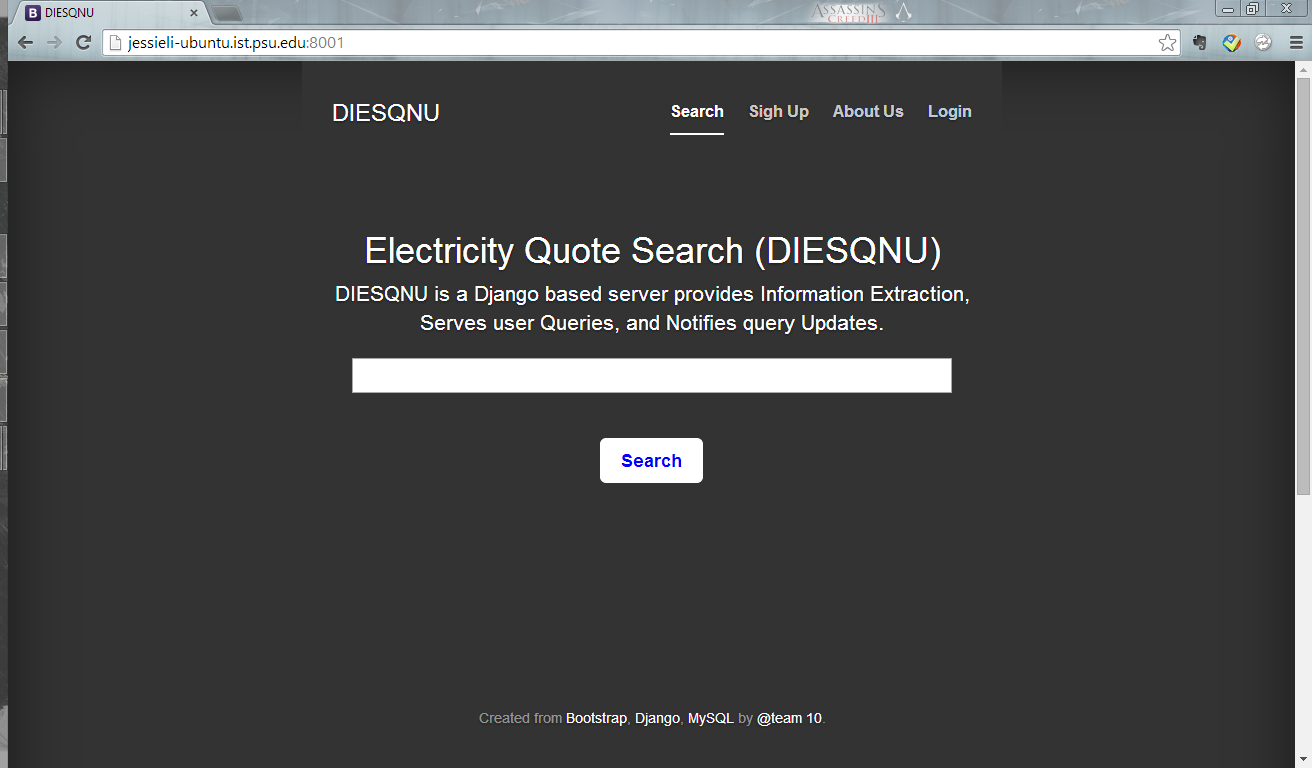
\includegraphics[width=0.7\textwidth]{fig/query.png}
\caption{Query page UI design.}
\end{figure}

\begin{figure}[h]
\centering
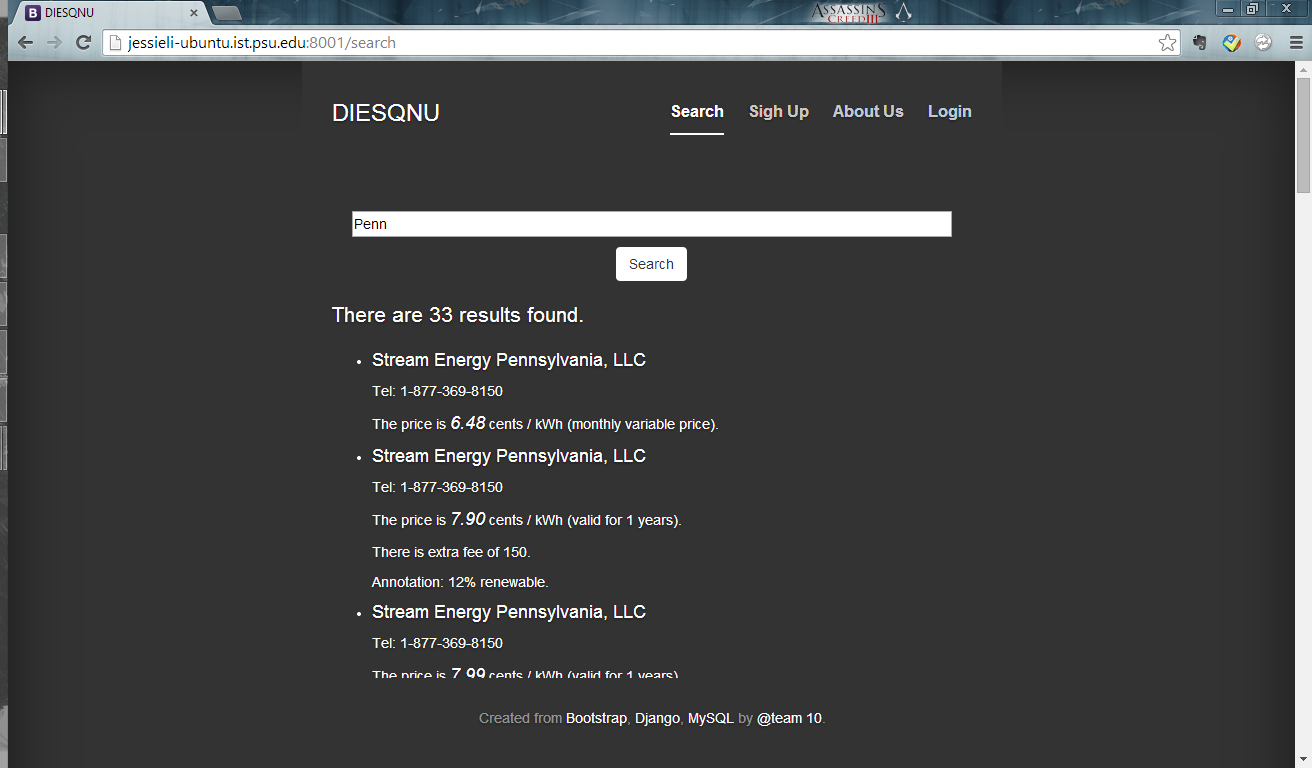
\includegraphics[width=0.7\textwidth]{fig/query-res.png}
\caption{Query results for keyword ``Penn''.}
\end{figure}


\subsection{User Registration}
User can registers in our web application and gets additional services such as the query change notification.

During the registration, system will check the availability of user name first, because no duplicated user names are allowed. Each entry in the sign-up table should be filled with correct information. Any mistakes in those fields will be notified to user.

\begin{figure}[h]
\centering
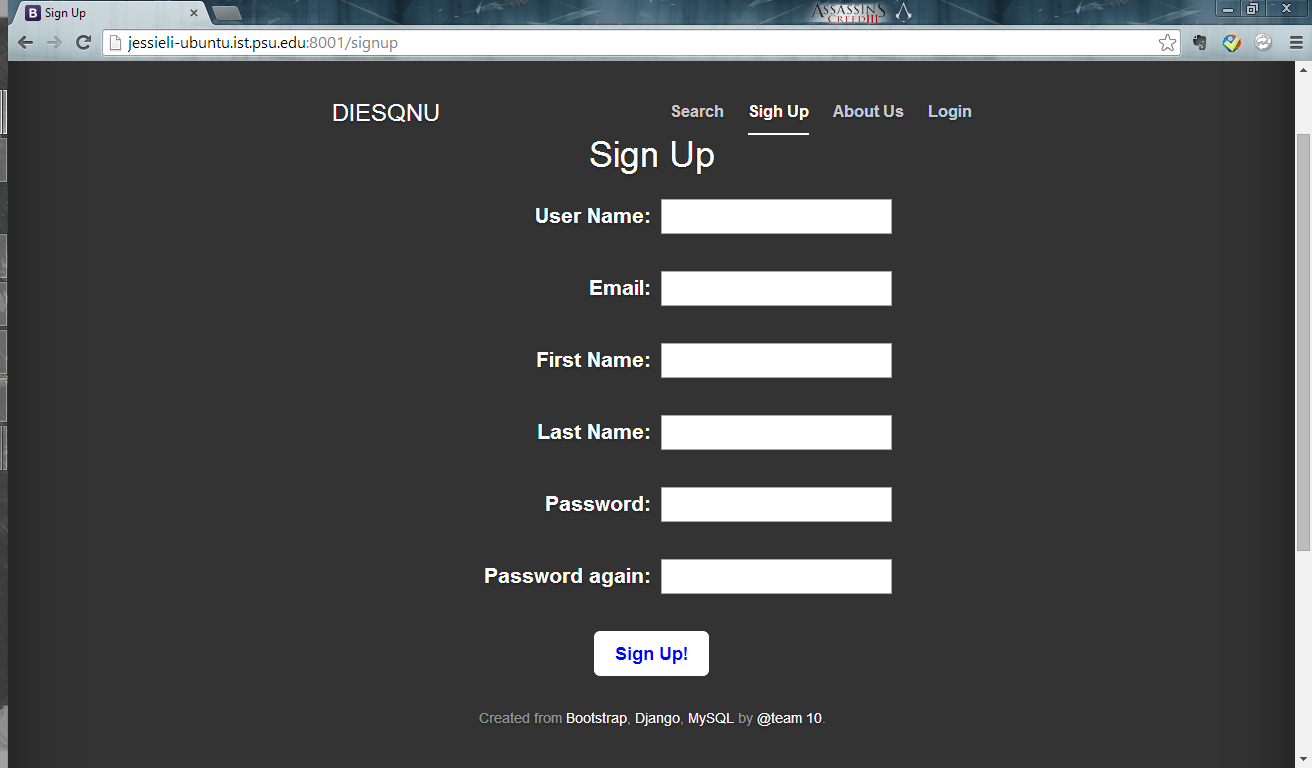
\includegraphics[width=0.7\textwidth]{fig/signup.png}
\caption{Sign up page for user.}
\end{figure}

\begin{figure}[h]
\centering
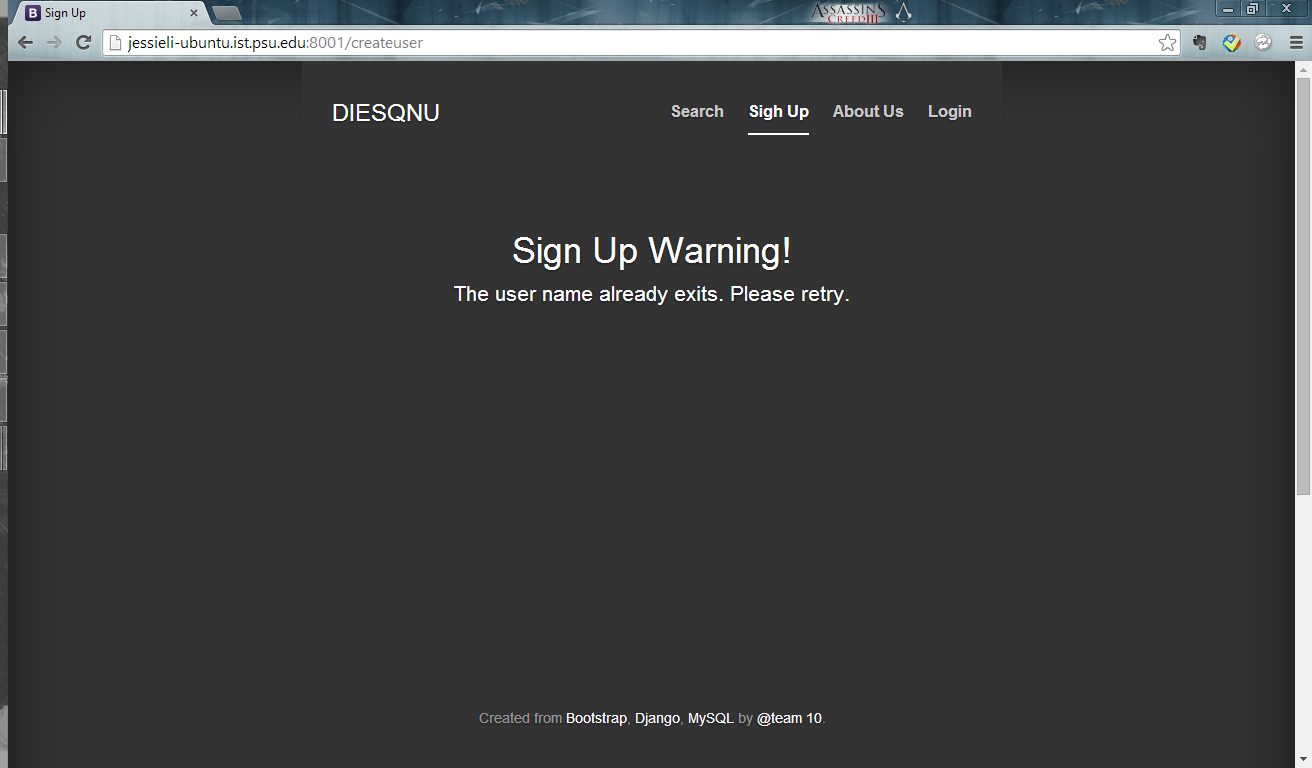
\includegraphics[width=0.7\textwidth]{fig/signup-error.PNG}
\caption{Sign up page result, when an error happens.}
\end{figure}


\subsection{User Login}
Registered user can login to our applications. Wrong passwords or in-valid user name will raise an error message.

After user logging in the web application, the sign in link will be replaced by a sign out link. There will be an additional welcome panel on the upper right conner of the page to notify the identity of logged user.

\begin{figure}[h]
\centering
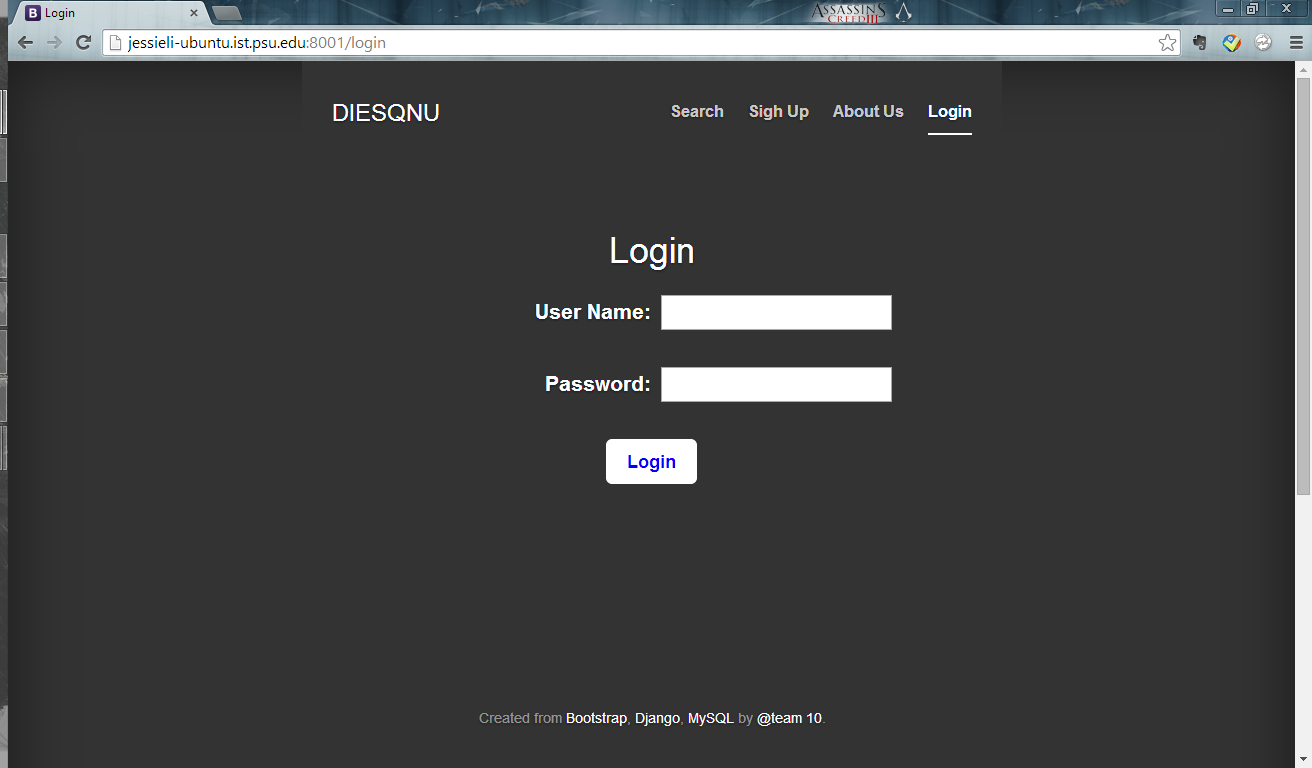
\includegraphics[width=0.7\textwidth]{fig/login.PNG}
\caption{Log in page for user.}
\end{figure}


\begin{figure}[h]
\centering
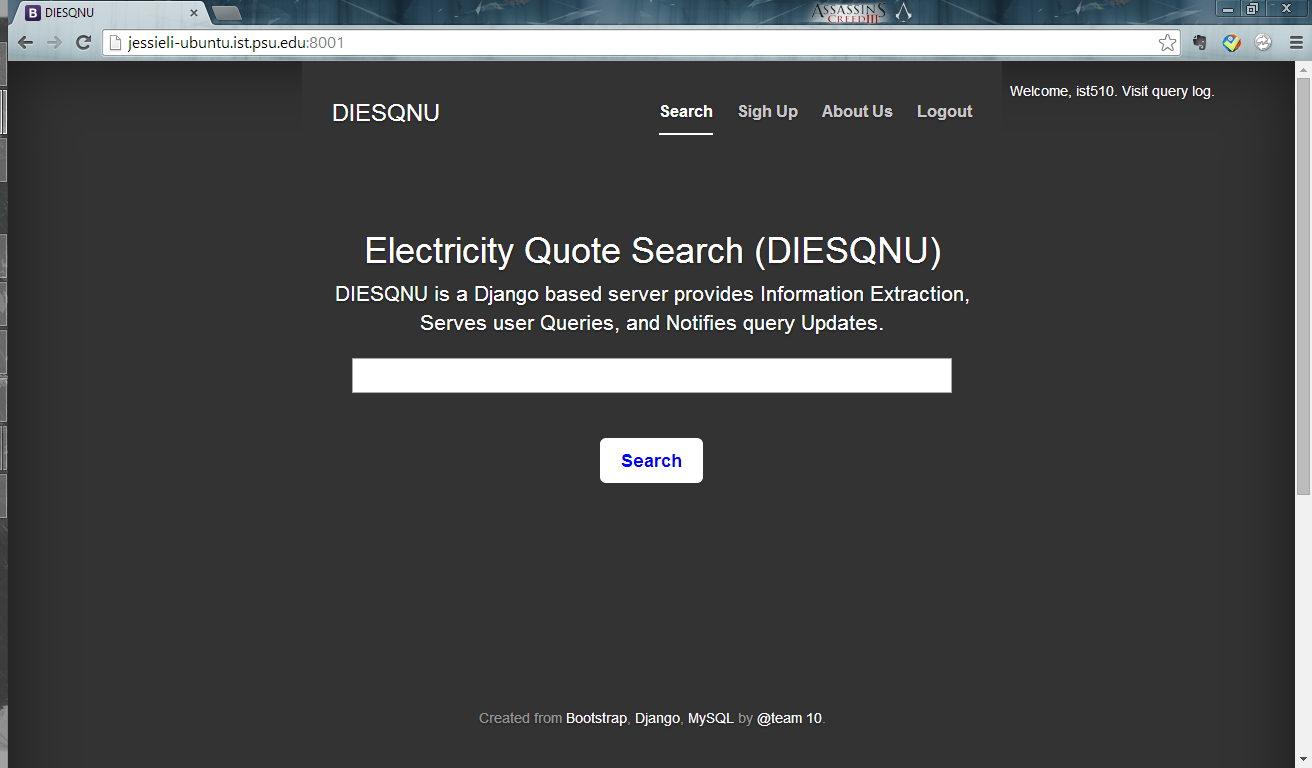
\includegraphics[width=0.7\textwidth]{fig/loggedin.PNG}
\caption{After user logged in application, there will be a welcome panel in the right conner.}
\end{figure}


\subsection{Query Log and Notification}

When user is logged into the web application, there is a link to the query log of the logged user in welcome panel. The query log page enables user to register query for change notification, as shown in Fig\,\ref{fig:not}.

In the query log page, we show the query string, time of that query, number of results and the registered status of that query. If the query is registered, the checkbox of this query is checked, and there is a link that allows us to unregister that query. On the other hand, if the query is not registered, we can check the unchecked box in front of it, and then using register query button to register it.

Notice that there is a ``check update'' button in the query log page. Our server will check the query changes periodically on the background. Here, for the sake of demonstration, we add a button to manually call this function. After calling the update check, the user can get the email notification, shown in Fig\,\ref{fig:email}.

\begin{figure}[h]
\centering
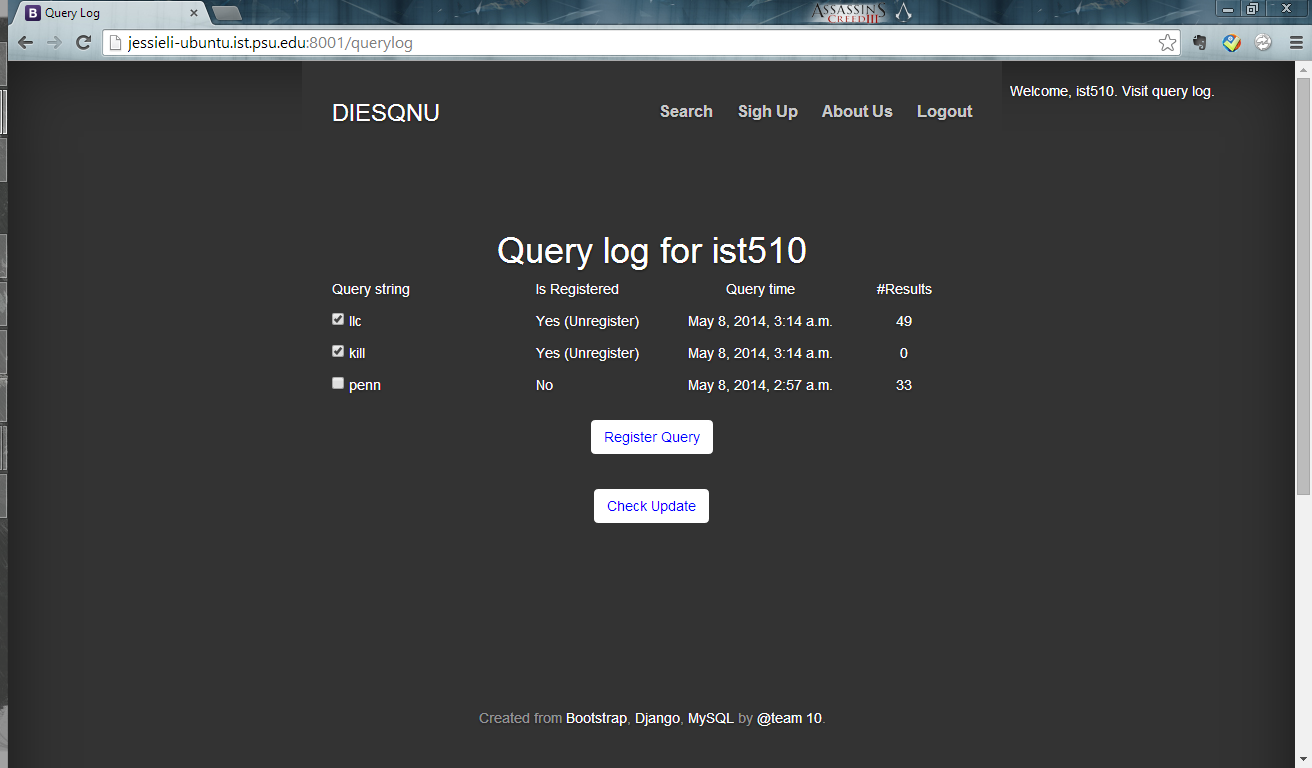
\includegraphics[width=0.7\textwidth]{fig/querylog.PNG}
\caption{The query log page, user can mange the query history from here.}
\label{fig:not}
\end{figure}


\begin{figure}[h]
\centering
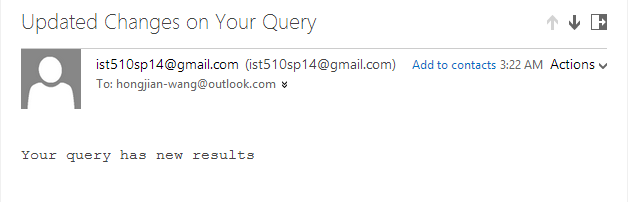
\includegraphics[width=0.7\textwidth]{fig/email-notification.PNG}
\caption{User can get email of query change notification.}
\label{fig:email}
\end{figure}


\subsection{Administration Console}

The Django framework provides us a free administration console, where we can directly see all the data in database and manipulate those data. A snapshot of this administration console is shown in Fig\,\ref{fig:admin}.

\begin{figure}[h]
\centering
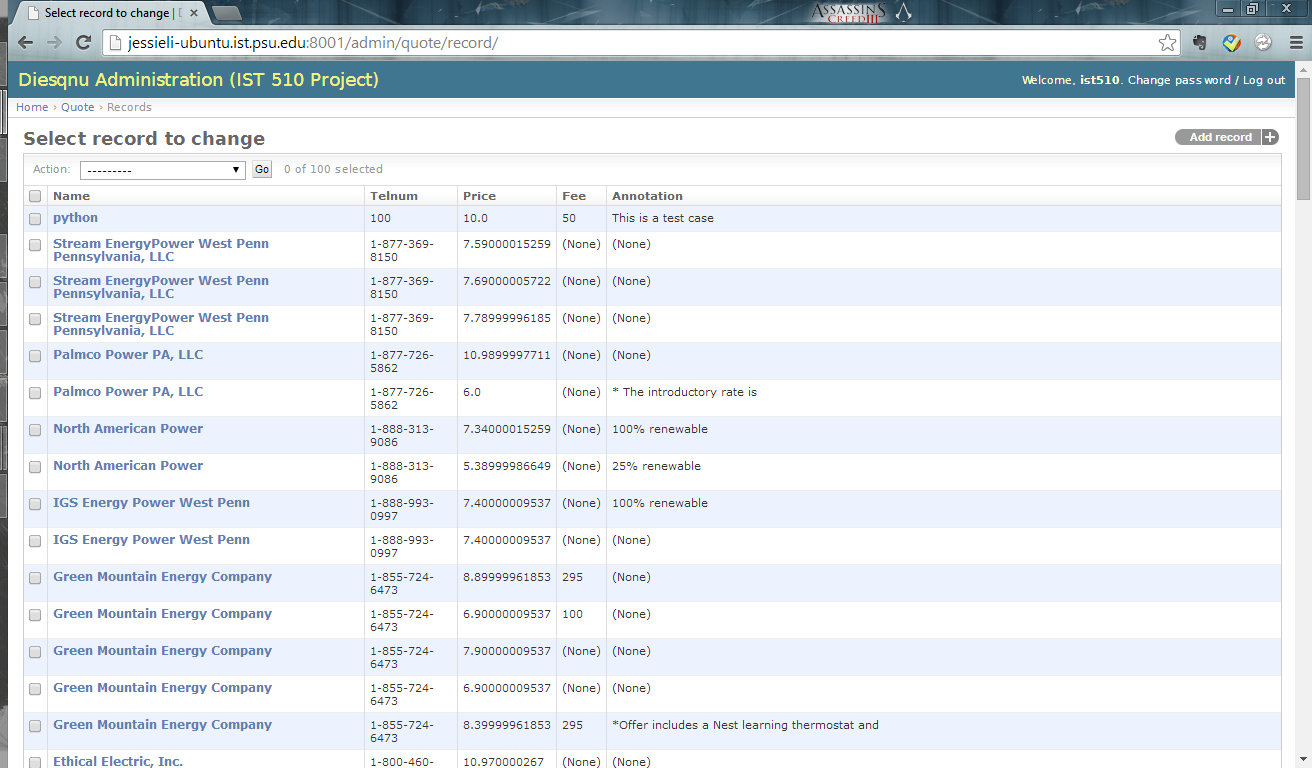
\includegraphics[width=0.7\textwidth]{fig/adminpage.png}
\caption{Administration console.}
\label{fig:admin}
\end{figure}




\section{Technical Details}

\subsection{Crawling}

add Dongpeng's part from Google doc.

\subsection{Identifying Changes and Sending Email Notification}

add Mohammad's part from Google doc.


\section{Conclusion}


\end{document}